\section{Validation}
\label{sec:evaluation}
In this section, we demonstrate by example that our algorithm satisfies the properties we set up as the goodness-of-split criteria for good small multiple displays.

%\begin{figure}[t]
% \centering 
%	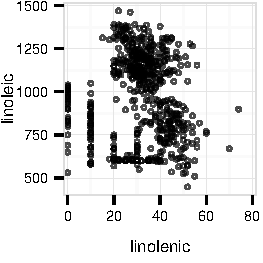
\includegraphics[width=1.75in]{images/linolenic-linoleic.pdf}
%	  \caption{An input scatterplot showing the relationship between two chemicals in the Olive oils dataset. There are strong, overlapping visual patterns in this data that our algorithm should be able to isolate. }
%	 \label{fig:vrich_all}
%\end{figure}
%
%\begin{figure}[t]
% \centering 
%	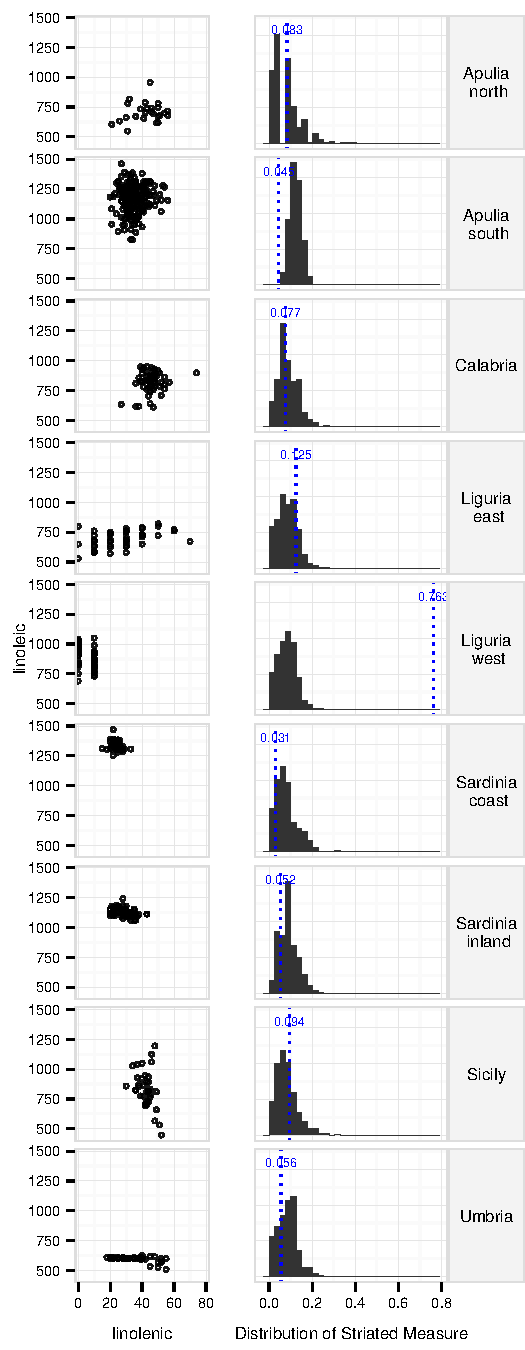
\includegraphics[width=3.05in]{images/15_729035813077-region.pdf}
%	  \caption{The highest ranked small multiple display of the olive oils data set using the striation scagnostic. Our algorithm detects that the striation pattern in Liguria west is very unlikely to be due to chance and recommends this small multiple display. }
%	 \label{fig:vrich_sm}
%\end{figure}

\begin{figure}[t]
 \centering
    \begin{subfigure}{1.05in}
	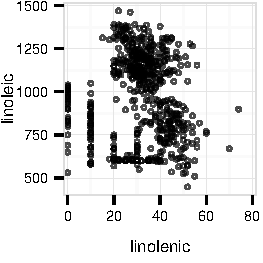
\includegraphics[width=1.05in]{images/linolenic-linoleic.pdf}
	  \caption{Input scatterplot}
	 \label{fig:vrich_all}
    \end{subfigure}
    \begin{subfigure}{2.5in}
	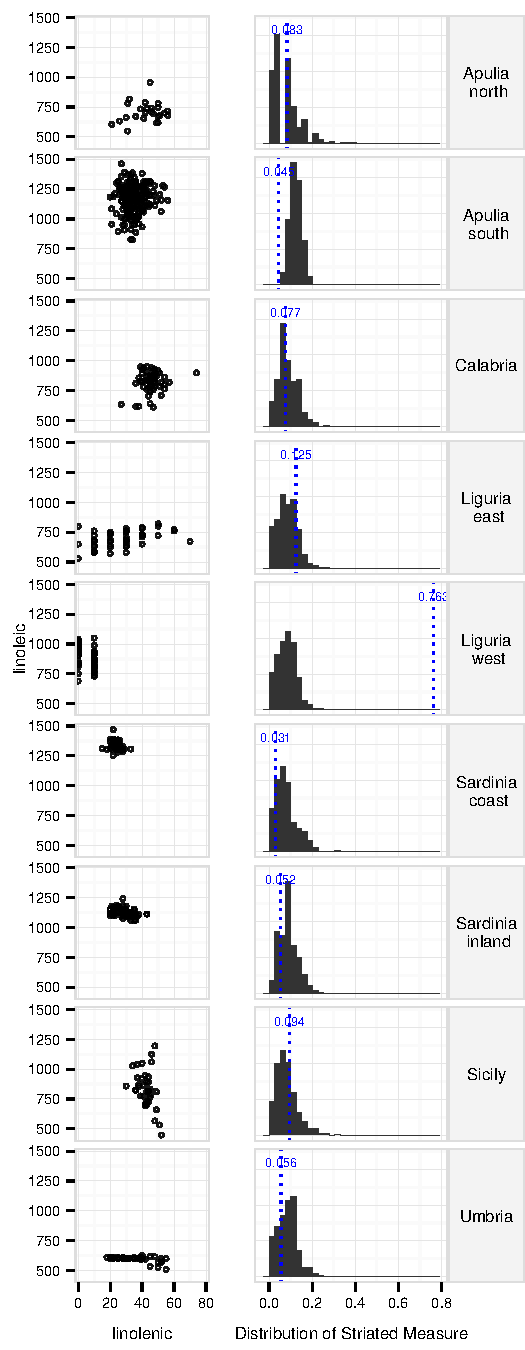
\includegraphics[width=2.5in]{images/15_729035813077-region.pdf}
	  \caption{Highest-ranked small multiple display}
	 \label{fig:vrich_sm}
    \end{subfigure}
	\caption{The highest ranked small multiple display of the olive oils data set using the striation scagnostic. Our algorithm detects that the striation pattern in Liguria west is very unlikely to be due to chance and recommends this small multiple display. }
\end{figure}

\subsection{Visually Rich}
Our first criterion is to prefer small multiple displays that have visually salient patterns. Our algorithm achieves this by using the input cognostic to measure the presence and extent of a visual pattern in the component plots of a candidate small multiple display. This approach works for arbitrary cognostic measures on any type of visualization, allowing us to create small multiple displays targeted at the interests of the analyst. 

For example, consider Figure~\ref{fig:vrich_all}, which shows the relationship between linolenic and linoleic in the olive oils dataset~\cite{Forina1983}, which includes eight chemical measurements on different specimens of olive oil produced in various regions in Italy. There are visually striking clumps and striation patterns in the data. An analyst might wonder whether these patterns can be isolated and explained by any of the other variables in the dataset.

To do so, the analyst can use our approach with Wilkinson et al.'s \emph{striation} scagnostic which detects banding of points in a scatterplot. With this cognostic, our approach ranks the ``Region" variable as the best partitioning variable for isolating striated patterns from the $p$ variables in the data set. This is the partitioning shown in the left half of Figure~\ref{fig:vrich_sm}, which reveals the clean isolation of the striation pattern for olive oils from the Liguria region and the distinctive measurement structure of linoleic values for the Umbria region.

As before, the right side of Figure~\ref{fig:vrich_sm} shows the true striation scores for this partitioning in blue and the randomized permutation scores in the black histogram. We can see that our algorithm has identified the striated pattern in Liguria west as being very unlikely to have arisen due to chance, leading to the top ranking for this small multiple. 
Note, however, that the striation in Liguria east is not identified as being an outlier. This is because the striation scagnostic itself fails to catch this case. Thus, the visual richness of the small multiples our approach selects depends on the quality of input cognostic, an issue we revisit in the discussion (Section~\ref{sec:discussion}).

\begin{figure}[t]
 \centering 
	 \begin{subfigure}{1.15in}
        \centering
		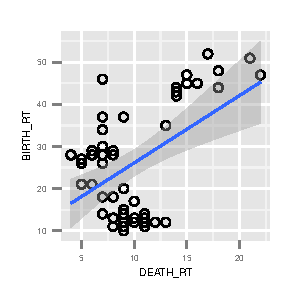
\includegraphics[width=1.15in]{images/DEATH_RT-BIRTH_RT.pdf}
		  \caption{Input scatterplot}
		 \label{fig:informative_all}
	\end{subfigure}
	\begin{subfigure}{3in}
		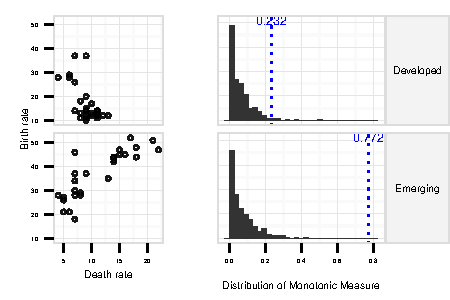
\includegraphics[width=3in]{images/9_95670214716782-GDP.pdf}
		  \caption{Partitioned by GDP category}
		 \label{fig:informative}
	 \end{subfigure}
	 \begin{subfigure}{3in}
		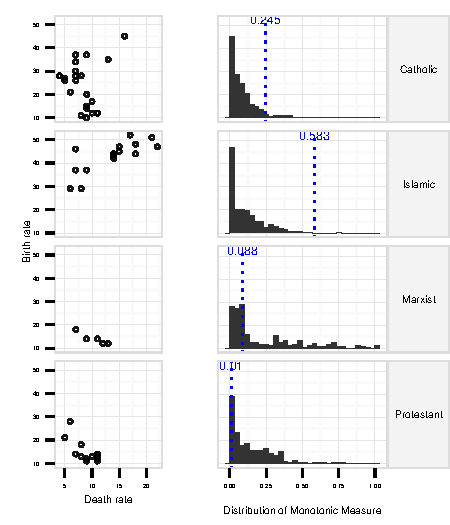
\includegraphics[width=3in]{images/3_80130820585327-LEADER.pdf}
		  \caption{Partitioned by the dominant religion}
		 \label{fig:not_informative}
	 \end{subfigure}
	  \caption{Our algorithm picks informative small multiple displays that diverge from the user-selected input plot. (a) User-selected relationship between birth and death rates for countries around the world. (b) The highest ranked small multiple display shows partitions that reveal strong opposite trends that were not seen in the original view. (c) The lowest ranked small multiple display that has more partitions with fewer points that look like random subsets of the input plot.}
\end{figure}

\subsection{Informative}
Our second criterion is that we want small multiple displays that reveal informative structures when compared to the original view. This criterion is incorporated in our algorithm by the comparison between the true cognostic score and that of the randomized permutations. Randomly permuting the partitioning variable results in partitions that are random subsets of the data in the original plot. Visual patterns in these random subsets are likely to be similar to those in the original plot, and thus, not informative. In contrast, a high absolute z-score for the true cognostic value is associated with a small multiple display that shows a pattern \emph{different} from the original plot.

An illustration of this behavior involves the Ourworld dataset of UN statistics on world countries~\cite{Wilkinson2005GG}. We want to determine how to partition the scatterplot showing the relationship between birth rate and death rate seen in Figure~\ref{fig:informative_all} to isolate the increasing and decreasing trends that seem to be overlaid. So we use the \emph{monotonic} scagnostic~\cite{Wilkinson2005} to find informative small multiples. The highest ranked small multiple is partitioned into two GDP categories, ``Developed" with $30$ points and ``Emerging" with $27$ points, as seen in Figure~\ref{fig:informative}. This partitioning reveals that GDP is a confounding covariate. While the main view shows an overall positive trend between the birth and death rates, the small multiple display shows that in developed regions there is only a strong negative relationship as expected for countries in that category. As shown by the histograms on the right, this informative display arises because the patterns in the small multiple display are substantially different from the patterns we would see in random subsets of the original plot.

Figure~\ref{fig:not_informative} shows the lowest ranked partitioning variable which categorizes countries by its dominant religion. This variable produces twice as many partitions with less visually salient monotonicity in those determined by ``Protestant" and ``Marxist" countries, particularly as the small number of points in each make the patterns seem more likely due to chance. %The visual patterns in the smaller partitions are barely informative because of their low support as discussed in the next section. 

%The negative correlation is contrary to the pattern in the original view. As such it is an example of Simpson's paradox when aggregate patterns are affected by changes in the relative size and value of the subpopulations. 


\subsection{Support}
Our third criterion for good small multiple displays is that they have patterns that are well-supported by the data. This property is incorporated into our approach through the use of the z-score normalization which adjusts for the variability in the simulated null distributions of the randomized cognostic scores. If the data set is small or there are outliers in the data set, this distribution will have high variance, which will downweight the resulting z-scores.

\begin{figure}
\centering
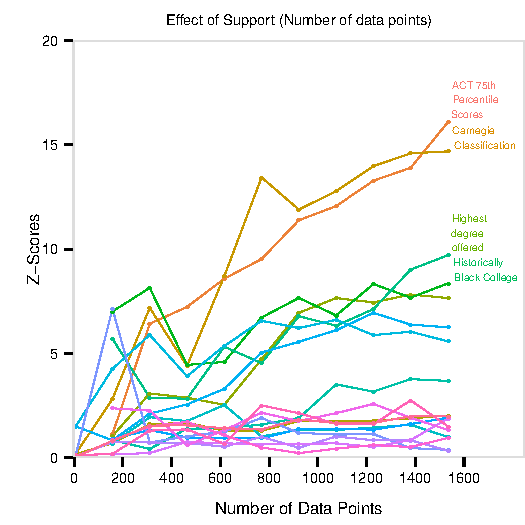
\includegraphics[width=3.25in,height=3.25in]{images/support-nogrid.pdf}
  \caption{The effect of support on the combined z-scores ranking of partitioning variables for the data about US universities. As the number of points in the dataset increases, the importance of the variable determined by the z-scores increases too. }
 \label{fig:support}
\end{figure}

To examine how our algorithm behaves with different amounts of support, we experiment by varying the size of the input data set. Using the US university data set discussed in the introduction and the monotonic scagnostic, we compute the z-scores for all the partitioning variables in the dataset. Figure~\ref{fig:support} shows these rankings for different data set sizes, generated by randomly subsetting the full data set.
As can be seen, for small data sets, the scores are small and, except for ACT scores, there is no clear ranking. The patterns in these small multiple displays are weaker and we correctly require more data to be confident in their ranking. As the data set grows, we become more confident in the rankings with ``Historically Black College'' and ``Carnegie Classification'' separating from the other variables. 
The smaller number of data points in the ``Yes" category of the small multiple display seen in Figure~\ref{fig:support1}, would make an analyst skeptical about any detected pattern, especially as the number of data points is reduced further. The visual pattern in the ``No" category exhibits some monotonicity but it looks similar to the original plot seen in Figure~\ref{fig:teaser1} and would not be very interesting.
The ``Carnegie Classification'' reveals a strong monotonic pattern in the partition determined by universities with very high research as seen in Figure~\ref{fig:support2}. However, this partitioning variable has a high cardinality, so, with fewer points in the dataset, the partitions it produces would have lower support making an analyst less confident of their validity.

\begin{figure}[t]
 \centering 
 	 \begin{subfigure}{2.5in}
 \centering 
		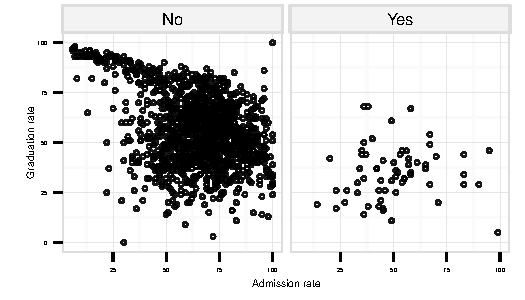
\includegraphics[width=2.5in]{images/Historically_Black_College.pdf}
		  \caption{Partitioned by whether universities were historically black colleges}
		 \label{fig:support1}
 	\end{subfigure}
 	 \begin{subfigure}{3.5in}
 \centering 
        \vspace{0.5cm}
		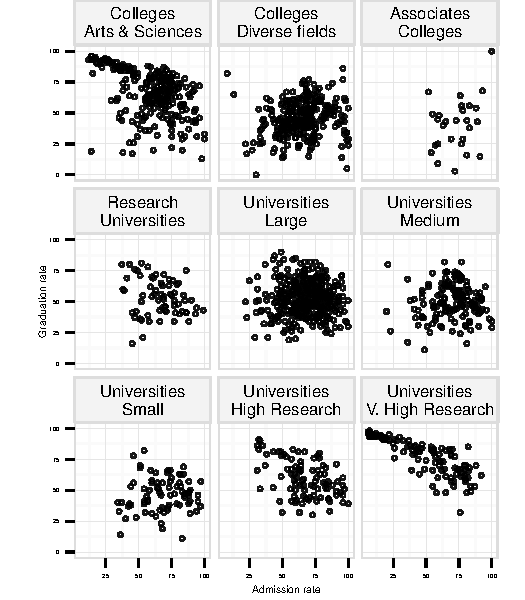
\includegraphics[width=3.5in]{images/Carnegie_Classification.pdf}
		  \caption{Partitioned by the Carnegie classification of universities}
		 \label{fig:support2}
 	\end{subfigure}
	\caption{Small multiple displays that are ranked higher as the size of the dataset increases. (a) Higher support promotes this small multiple defined by the ``Historically Black College" variable as the pattern in the smaller partition becomes more important. (b) ``Carnegie Classification'' produces many partitions with low support. Increasing the size of the dataset increases the support of the highly monotonic pattern raising the rank of this small multiple display.}
\end{figure}


\subsection{Parsimonious}
  \begin{figure}[t]
    \centering
    \begin{minipage}[b]{1.7in}
       \begin{subfigure}[b]{\linewidth}
        \centering
  	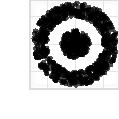
\includegraphics[width=0.85in]{images/donut1-donut2.pdf}
        \vspace{-0.5cm}
      \caption{Input bullseye scatterplot}
      \label{fig:pars1}
      \end{subfigure}\\[\baselineskip]
      \begin{subfigure}[b]{\linewidth}
  	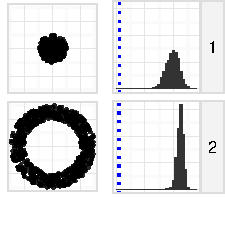
\includegraphics[width=1.65in]{images/19_5065416601259-cluster.pdf}
        \vspace{-0.5cm}
      \caption{Bullseye split into 2 partitions}
        \vspace{0.25cm}
      \label{fig:pars2}
      \end{subfigure}
      \begin{subfigure}[b]{\linewidth}
  	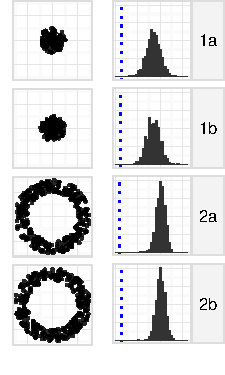
\includegraphics[width=1.65in]{images/9_27395081160431-cluster1.pdf}
        \vspace{-0.5cm}
        \caption{Bullseye split into 4 partitions}
      \label{fig:pars3}        
      \end{subfigure}
    \end{minipage}
    \begin{subfigure}[b]{1.7in}
	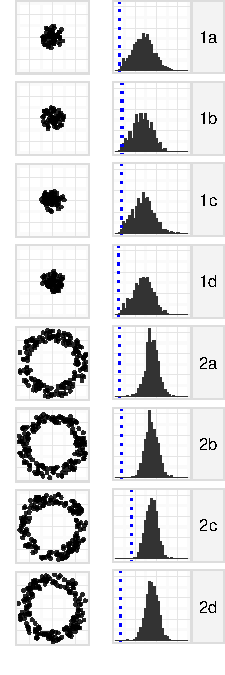
\includegraphics[width=1.7in]{images/5_12851615653375-cluster2.pdf}
        \vspace{-0.5cm}
      \caption{Bullseye split into 8 partitions}
      \label{fig:pars4}
    \end{subfigure}
    \caption{Our ranking of small multiple displays of an artificially generated data pattern respects the parsimony criterion. (a) The input bullseye pattern. (b) The best small multiple display determined by the clumpy scagnostic. (c) The second best partitioning variable redundantly halves the two partitions from (b). (d) The lowest ranked small multiple display with eight partitions.}
    \label{fig:parsimonious}
  \end{figure}

Our final criteria is parsimony. This criteria is indirectly included in our approach. High-cardinality variables create a large number of partitions, which are likely to have low support as the observations get distributed among more partitions. Thus, we will tend to reject such partitionings if more parsimonious options are available.
 
We illustrate this behavior using an artificially generated dataset so we can hold the visual patterns across partitioning variables equal as far as possible. The input visualization is the bullseye pattern shown in Figure~\ref{fig:pars1}. This artificial data set includes a partitioning variable that cleanly separates the ring from the core as seen in Figure~\ref{fig:pars2}. It also includes two other partitioning variables that separate the ring and core, but they further split them into two and four random partitions (Figures~\ref{fig:pars3} and~\ref{fig:pars4}). The separation between the core and ring are equally visible in all three variants, however the first is the most parsimonious---it shows the pattern in the fewest number of component plots. 
To discover such partitionings of the visual pattern, we could use Wilkinson et al.'s \emph{clumpy} scagnostic that has high values for scatterplots with multiple tight clumps of points. So, plots of random samples of the bullseye pattern will produce a distribution of clumpy scores that are high but the plots that split out the core and the ring will have clumpy scores that are much lower.

In the histograms, we can see that the width of the distributions increases as the number of partitions increases. Thus, the computed z-score will be highest for the first partitioning variable. The actual values are $19.507$, $9.274$ and $5.129$ for Figures~\ref{fig:pars2},~\ref{fig:pars3} and~\ref{fig:pars4}. Thus, our approach does prefer more parsimonious partitioning variables.

